\chapter{Diseño de la Solución} \label{Diseño de Solucion}
%Brindar una respuesta a los requerimientos de la sección anterior.
En base a los requerimientos analizados en la sección anterior, en esta sección se detallan las decisiones tomadas de forma de brindar una respuesta a los mismos. 
Primero se describen las decisiones con respecto a los elementos del dominio, esto es, que elementos se van a considerar para los siguientes pasos, a partir de esto se describe el modelo UML que será la base del proyecto, y finalmente se definen las herramientas que se utilizarán como soporte para poder cumplir con el resto de requerimientos, es decir, la transformación y aplicación de archivos de configuración.

\section{Definición de Dominio Específico}
Partiendo de que el objetivo del proyecto es ofrecer la capacidad de modelar la configuración de una red de dispositivos, se tiene que los conceptos claves a modelar son los dispositivos y la configuración aplicada a los mismos.
Esto también se puede ver como la topología de la red, es decir, los nodos que se encuentran en la red a modelar, y la configuración aplicada a dicha red y sus respectivos dispositivos o nodos.

La topología de red puede verse desde dos enfoques: el enfoque físico y el lógico, de los cuales se desprenden los conceptos de nodo físico y nodo lógico. Se consideran nodos físicos a los dispositivos en sí, como lo son las computadoras o routers, con el fin de representar de forma precisa los diferentes dispositivos físicos que se encuentra en la red. Por otro lado, se consideran nodos lógicos a los componentes que se encuentran en los nodos físicos, estos van desde sistemas operativos hasta programas de software instalados, ya que el objetivo es representar el estado del dispositivo de forma tan precisa como sea posible.
Con estos elementos se obtiene una imagen o descripción general de los nodos presentes en la infraestructura de la red.

\subsection{Nodos Físicos}
Desde el punto de vista de los nodos físicos, los componentes a modelar serán los dispositivos de red, es decir, los routers y switches, los servidores, las computadoras personales (pc o workstation), y por último el resto de dispositivos que se puedan conectar a una red, como puede ser una impresora o un escáner de red. A estos últimos los denominaremos con el término genérico de "dispositivos".

Se consideran estos componentes por ser los básicos y más usuales que se encontrarán en una red, cubriendo así la mayoría de los escenarios posibles. Los dispositivos de red son la base para un sistema de este estilo, por lo que es imprescindible que \textbf{Router} y \textbf{Switch} sean representados. Luego es necesario hacer una distinción entre \textbf{Servidor} y \textbf{PC}, ya que cumplen funciones diferentes e interesa representar esta diferencia en el lenguaje. Además en la mayoría de los casos se encontrarán en diferentes cantidades.
Finalmente se tiene el componente \textbf{Dispositivo} para encapsular al resto de componentes y poder representar de forma más fiel la realidad del sistema estudiado.

\subsection{Nodos Lógicos}
En el caso de los nodos lógicos, interesa saber el \textbf{Sistema Operativo} de los \textbf{Servidores} y \textbf{PC} por un lado, y el \textbf{Firmware} de los nodos de red por otro lado. Asimismo, se debe tener en cuenta el software instalado en cada componente, en particular en los \textbf{Servidores} y \textbf{PCs}, por lo que deberán ser contemplados en el modelo. 

Los componentes de software considerados para modelar son los siguientes: 
\begin{itemize}
    \item un componente de \textbf{Firewall}
    \item un ambiente de ejecución (\textbf{Runtime}), en este caso se consideró el de \textbf{Java}
    \item un servidor de aplicaciones (\textbf{Application Server}), \textbf{Tomcat} en este caso
    \item un servidor HTTP (\textbf{HTTP Server}), para el que se utilizará \textbf{Apache}
    \item motores de bases de datos (\textbf{Database Engines}), para los cuales se representará \textbf{MySQL} y \textbf{PostgreSQL}
\end{itemize}

La decisión de estos componentes se basa en tener diferentes clases de componentes, y que a la vez sean normalmente utilizados por CMTs (Configuration Manager Tools), la importancia de esto se explicará en detalle en la sección \textbf{CMTs a Utilizar}. También es necesario acotar la cantidad de componentes de software ya que estos deberán ser modelados, y siendo esta una primer iteración del objetivo, tendrá más importancia obtener una prueba de concepto, que luego pueda ser extendida fácilmente con más componentes.

\subsection{Configuración}
La configuración es el punto más importante, y que mayor valor da al proyecto, ya que la transformación se basará principalmente en este componente y en los componentes lógicos de software para generar los scripts de configuración, los que finalmente serán utilizados para aplicar el estado a la red.
Por esto, es importante que se contemplen la mayor cantidad de escenarios posibles de configuración.
Al igual que con los componentes de software, parte de la decisión se basa en el uso de CMTs (Configuration Manager Tools), que se explicará en detalle en la sección \textbf{CMTs a Utilizar}.

En este caso se definen tres clases de configuración en función de las características y la relación con el resto de los elementos.
Primero se tiene la \textbf{configuración de software}, esta clase se corresponderá con los componentes de software definidos como nodos lógicos. Los elementos de este tipo son específicos a cada componente de software ya que representan los aspectos configurables particulares de cada software que se desea configurar.

Luego se define la \textbf{configuración de archivo}, nombrada de esta forma por ser análoga a la función que cumple dicha configuración en los CMTs, esto es, acciones discretas sobre archivos del sistema, por ejemplo: verificación de presencia o contenido, copiado o borrado de dichos archivos, etc. Este tipo de elemento es muy importante ya que, en ausencia de un elemento de software o configuración del mismo se puede recurrir a manipular directamente archivos para llevar a cabo una configuración.

Finalmente, se tiene una configuración libre, cuyo propósito es la de dar la oportunidad de registrar cualquier tipo de configuración que no pueda ser aplicada de forma automática por las herramienta, pero que podría interesar guardar un estado, como lo son los componentes \textbf{Dispositivos}. De esta forma, se pueden modelar opciones de configuración que no estén soportadas por un CMT, o cualquier comentario que se desee guardar en el correspondiente nodo. 
Un ejemplo de esto puede ser la configuración de una impresora: las impresoras en general no proveen un sistema de configuración automática y se debe realizar la misma de manera manual. Con un elemento de configuración libre se puede asociar a la impresora una lista de los distintos valores a configurar, un tutorial o un link a una guía de configuración.

De forma similar, pero sólo aplicable en el caso de sistemas operativos Windows, se tiene una cuarta clase de configuración llamada \textbf{Registro (Registry)}, que como el nombre lo indica, son configuraciones que pueden ser aplicadas al registro de Windows. Esta última clase es necesaria ya que una gran cantidad de configuraciones en Windows se realizan a través de sus registros.

\section{Lenguaje de Modelado del Dominio}
%Descripción de cada elemento generado.
%Descripción del metamodelo UML final implementado, explicando en detalle y justificando decisiones.

\subsection{Lenguaje a Utilizar}
Antes de comenzar con la implementación del modelo, es necesario elegir el lenguaje que se va a utilizar. En este sentido hay dos grandes opciones, por un lado se tienen los lenguajes de dominio específicos o DSL por sus siglas en inglés (Domain Specific Languages), y por otro lado se tienen los perfiles UML. 

Los DSL son utilizados para resolver un problema en particular, y representan un problema o dominio específico, como su nombre lo indica.
Los perfiles UML, tal como se detalló en la introducción, se utilizan para extender modelos UML para ciertos dominios o plataformas.
En base a estas descripciones, se puede ver que ambos lenguajes serían apropiados para cumplir con el fin de representar la realidad planteada. 

En este caso, luego de analizar diferentes ventajas y desventajas de ambos, se optó por utilizar el perfil UML. La principal razón de la decisión se basa en que una gran parte de lo que se quiere representar, como el caso de la topología, ya posee contraparte en UML, por lo que sería favorable partir de esta base. 

Sucede lo mismo con los diagramas de deployment de UML, su representación de nodos y componentes que se ejecutan en dichos nodos, se ajusta a la descripción del problema planteado, por lo que se puede tomar ventaja de dichos elementos y reutilizarlos para la implementación de la solución.

Otra razón para esto es la estandarización de UML comparado a un DSL. Al extender UML se puede hacer uso de todas las herramientas ya existentes para dicho lenguaje, mientras que para un DSL se deberían implementar todo un ecosistema análogo. Al elegir UML como base ya se tienen editores, mecanismos de extensión y una sintaxis en la cual basarse.

Finalmente, si se piensa en la implementación es posible ver una analogía entre elementos existentes de UML y el problema que se intenta resolver, que servirán al momento de definir la extensión, esto es, el concepto de \textbf{Nodo} y \textbf{Deployment} que posee UML. 

En primer lugar, según la especificación formal de UML \cite{UML}, el elemento \textbf{Nodo} se divide en dos especializaciones, por un lado \textbf{Device} representa componentes de máquinas físicas, que coincide con el concepto de nodo físico; y por otro lado \textbf{ExecutionEnvironment}, se asignan a componentes de Device, y representan sistemas de software estándar, lo que es análogo a lo que se definió como nodo lógico. 

Por otro lado, el elemento \textbf{Deployment} representa las relaciones entre elementos físicos y lógicos de un sistema, así como características asignadas a estas relaciones. En este caso, el nodo lógico que se menciona en la especificación coincide con nuestro concepto de configuración.

La representación de UML para el elemento \textbf{Node} es capturada en la Figura \ref{fig:requirements:uml_node}, mientras que la representación de \textbf{Deployment} es capturada en la Figura \ref{fig:requirements:uml_deployment}.

\begin{figure}[H]
    \centering
    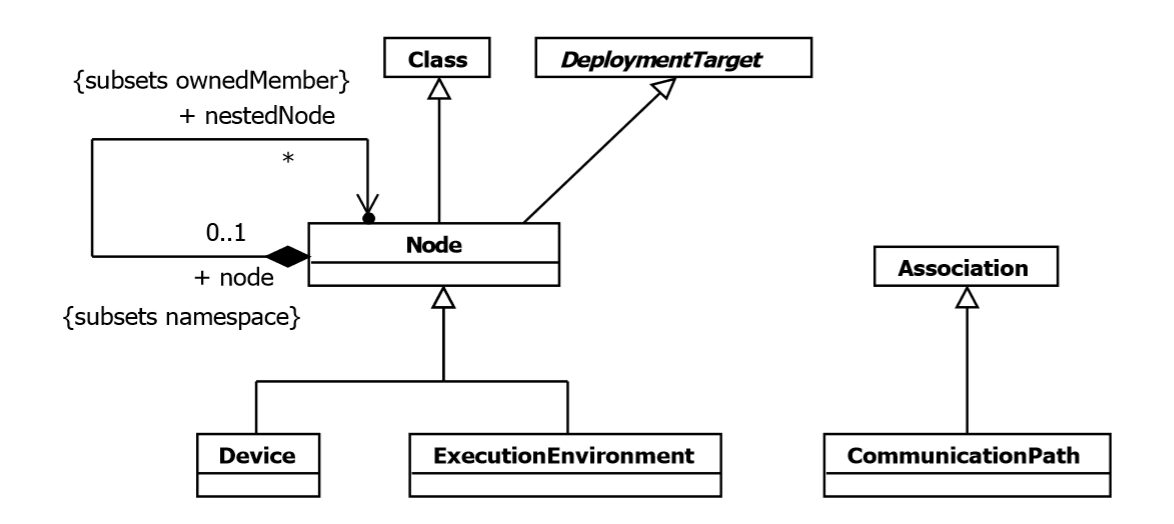
\includegraphics[width=0.75\textwidth]{figures/requirements/node_device_exec.png}
    \caption{Representación de UML de Node.}
    \label{fig:requirements:uml_node}
\end{figure}

\begin{figure}[H]
    \centering
    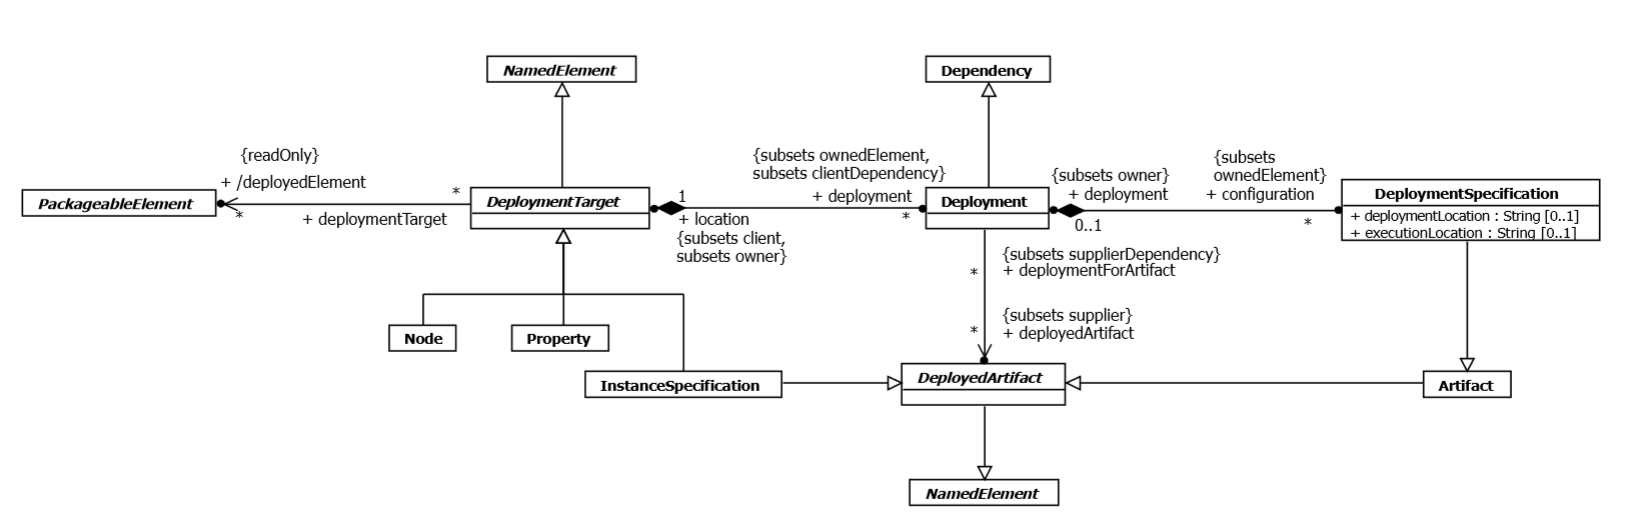
\includegraphics[width=\textwidth]{figures/requirements/deployment_syntax.png}
    \caption{Representación de UML de Deployment.}
    \label{fig:requirements:uml_deployment}
\end{figure}


El conjunto de estas ventajas, y en particular las similitudes encontradas entre los componentes definidos por UML y la realidad que se desea resolver, llevaron a optar por la creación de un perfil UML, en lugar de utilizar un DSL.

\section{CMT a Utilizar}

Otro paso fundamental en el diseño de la solución es la elección de la herramienta de configuración a utilizar. Una posibilidad era utilizar un Configuration Manager Tool que se encargue de la configuración de los nodos y de la red, y éste fue el camino por el que se optó. 

La principal ventaja de estas herramientas es que utilizan scripts con un formato específico para realizar la configuración, lo que es sumamente importante al momento de generar dichos archivos, ya que se tendrá un formato definido y único. Otra ventaja de gran valor es que dichas herramientas centralizan la configuración, lo cuál era una de las características claves que se analizaron en capítulos anteriores.

Con esta decisión tomada, el siguiente paso es la elección de los CMTs a utilizar. En este paso se analizaron una variedad de CMTs, entre los cuales destacaron Puppet, Chef y Ansible. Finalmente se decidió decantarse por el lado de Puppet o Chef, ya que ambos pertenecen a lo que se podría denominar una misma familia de sistemas de manejo de configuración: ambos tienen un lenguaje declarativo que describe el estado de un sistema y apuntan a su uso durante todo el ciclo de vida del mismo. Ansible por el otro lado se enfoca más en el principio de este ciclo, en la etapa de aprovisionamiento de servidores, con lo cual mantener el estado más allá de esta etapa implicaría trabajo extra con respecto a Puppet/Chef, aunque de todos modos sería posible.

Finalmente se eligió Puppet como objetivo principal ya que si bien tanto Puppet como Chef son herramientas líderes en el mercado \cite{puppetmarket}, debido a la familiaridad del equipo con el primero se consideró que sería más sencillo utilizarlo. Adicionalmente ambos son tan similares (estructuras de directorios, archivos de configuración, sintaxis, arquitectura) que no se consideró que realizar transformaciones para ambos agregara valor.

\section{Transformación M2T}

Finalmente se debió diseñar la transformación M2T que tomará el modelo de la realidad, y tendrá como salida la configuración necesaria para que el Puppet Master pueda impactar el estado deseado en la red.

Para cada elemento del dominio específico se generará un archivo. Dichos archivos se organizarán en una estructura de directorios arborescente, donde se diferenciarán en tres clases, y dentro de cada clase se organizarán en base a cada elemento y sus relaciones.
De este modo se tiene una gran modularidad y simplicidad en cada archivo, ya que en el mismo sólo se indican las propiedades del elemento correspondiente, y se apunta a otros archivos de similar complejidad.

En lineas generales, se plantean las siguientes reglas:
\begin{itemize}
    \item En primer lugar se genera un archivo site.pp donde se listan todos los nodos físicos que permitan una configuración. Para cada nodo se genera una expresión regular y se le asigna una clase propia.
    \item Para cada nodo físico se genera un archivo cuyo contenido son \textit{includes} de las clases generadas para los nodos lógicos pertenecientes a dicho nodo físico. Este archivo se ubica en un directorio llamado "device"; también se crea un directorio con el nombre del nodo físico, que contendrá los archivos generados por sus nodos lógicos asociados.
    \item De similar manera, para cada nodo lógico se genera un archivo cuyo contenido son los valores básicos de la instalación del mismo, así como \textit{includes} para las configuraciones asociadas. Este archivo se ubica en el directorio previamente creado para el nodo físico correspondiente; al mismo tiempo se crea un directorio dentro del directorio "configuration" con el nombre del nodo lógico, que contendrá los archivos asociados a los elementos de configuración de este nodo.
    \item Luego, para cada configuración se genera un archivo con los valores de la misma. El archivo se ubica dentro del directorio del nodo lógico correspondiente, creado previamente en el directorio "configuration".
    \item Finalmente, para cualquier elemento que no corresponda crear un script de configuración, se crea un archivo de texto plano con su información en forma de clave valor, este archivo tendrá el nombre del elemento, y se ubicará en el directorio del nodo físico correspondiente (su propio directorio en caso que sea un nodo físico), dentro del directorio "information".
\end{itemize}

Un ejemplo de esta estructura puede ser el que se encuentra en la Figura \ref{fig:requirements:file_structure}.

\begin{figure}[H]
    \centering
    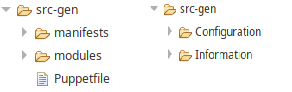
\includegraphics[width=0.5\textwidth]{figures/requirements/structure.png}
    \caption{Ejemplo de estructura de archivos generados.}
    \label{fig:requirements:file_structure}
\end{figure}

%En cierto punto decidimos utilizar los CMs del estilo Puppet, Ansible, Chef. 
%Podemos profundizar lo hablado en la introducción, describiendo como funcionan al detalle, esto es necesario ya que utilizamos esto para crear las transformaciones.
%Explicación de cómo se integra con la implementación del perfil y la generación de la transformación.
%Aca tambien podemos mostrar ejemplos de modulos de Puppet o Chef.



%%% Local Variables:
%%% TeX-master: "../main"
%%% End:
